\documentclass{article}
\usepackage[utf8]{inputenc}

\title{Part 1 - Author Interest Diversity}
\author{Ella Guest}
\date{February 2019}

\usepackage{natbib}
\usepackage{graphicx}
\usepackage{booktabs}
\usepackage{xcolor}
\usepackage{caption}
\usepackage{subcaption}
\usepackage{amsmath}
\usepackage{lscape} 
\usepackage{hyperref}


\begin{document}

\maketitle

\tableofcontents

\listoffigures
 
\listoftables

\section{Methodology Overview}
\begin{itemize}
    \item understand how subreddit communities vary in the extent to which they engage with a diverse range of subreddits
    \item most measures in this section are performed at the author-level, and then aggregated by subreddit
\end{itemize}


\subsection{How does interest diversity vary between subreddits }
For each author I will calculate the number of subreddits they commented in and b) the comment entropy. The subreddit count will give a general idea of author activity on Reddit. The comment entropy will give a better understanding of how equally authors divide their contributions across the subreddits they frequent.


\subsection{How do ‘chamber’ members concentrate within the chamber?}

The literature on echo chamber suggests that confirmation bias encourages people to enter and maintain echo chambers, as we experience pleasure from having our opinions re-affirmed by a group. To test this hypothesis I will determine whether authors who choose to comment in the case study echo chamber spend relatively more time within the chamber than authors in other subreddits. This research question has two sub questions.

\subsubsection{Do chamber members spend more time within the chamber than members of other communities?}

To test this I will measure the in-subreddit ratio for each author, for each subreddit they comment in. The in-subreddit ratio is the number of comments made within the subreddit as a fraction of the total number of comments the author made.

\subsubsection{How does author activity vary within subreddits}

The literature suggests that the majority of participation in online communities is heavily unequal. I seek to determine whether this phenomenon hold for echo chambers. I suggest two two possible scenarios: a) chambers are more unequal as they have a more active core of devoted members, or, conversely b) they are more equal as their members are generally equally devoted. I do not yet have a working hypothesis based on the literature on which direction echo chamber participation should be theorised to lean, though my intuition is A.

To measure participation inequality I will first use the same entropy measure from 1.1. This subreddit author entropy will look at the range in number of comments made by all authors. I will then use a more traditional measure of participation inequality, though I have not yet determined which. Options include the gini coefficient and the Pareto principle but I need to do a small literature review to determine which measure has been most appropriately and successfully used for online communities.


\subsection{Diversity Measures} \label{subreddit vector}
For each subreddit $s_i$ there are $n$ comment authors. For the $nth$ author in subreddit $s_i$ there are $x_n$ number of comments, such that for each subreddit we have the vector:

$$s_i = [x_1, x_2, \cdots x_n]$$

I then use this vector to calculate each of the diversity measures (entropy, blau, gini).


\subsubsection{Entropy} \label{entropy}

"Information entropy is the average rate at which information is produced by a stochastic source of data." The lower the probability of a value, the greater the "information" it carries. The higher the entropy, the greater the disorder or uncertainty.

Within the context of subreddits, if an author only makes a few comments in the subreddit, any new content they bring to subreddit provides relatively more information... Therefore the higher a subreddit's entropy the greater the diversity...


$$Entropy = -\sum p_ilog(p_i)$$

where $p_i$ is the probability of value $x_i$;

$$p_i = \frac{x_i}{\sum x}$$

The maximum entropy for a subreddit is $log(n)$ thus be can normalise entropy as:

$$Entropy_{norm} = \frac{Entropy}{log(n)}$$

\subsubsection{Blau index} \label{blau index}

The Blau index is also known as the Gini-Simpson index, or the Gibbs-Martin index. The Blau index of diversity has a range of 0 to 1, where 0 means the population is perfectly homogeneous, and 1 means the population if perfectly heterogeneous. Therefore the higher the a subreddit's blau, the more heterogeneous the distribution of comments amongst authors, the greater the diversity.


\textcolor{red}{Need to look into using 'true diversity' or normalised blau - may be more informative for more active subreddits (and more correlated to entropy). Can the "effective number of types" show a diversity threshold?}

$$Blau = 1 - \sum (\frac{x_i}{\sum x_n})^{2}$$

\subsubsection{Gini coefficient} \label{gini}

The gini coefficient is a measure of inequality in a distribution. It is a ratio between the values of 0 and 1, where 0 means perfect equality and 1 means perfect inequality. Therefore the higher the value of gini for a given subreddit, the more unequally comments are distributed across authors within the subreddit.

$$Gini = \frac{1}{n}(n+1-2\frac{\sum(n+1-i)y_i}{\sum y_i})$$





\section{General Diversity Trends} \label{1.1}

The example findings are from February 2018, until I re-run the rest of 2018. In February 2018 86,467,179 comments were made across 104,042 subreddits by 4,282,601 authors. At least 6.1\% of comments were later deleted (N=5,317,239).

Table \ref{table/all} shows that at least half of subreddits had 3 or fewer unique comment authors in February 2018, and 4 or fewer comments. For both count measures the upper quartile is still smaller that the maximum values. I therefore decided to subset the top decile of subreddits by author count as active communities.


\subsection{Default Subreddits}
50 subreddits were at one time classified as a default. Any new redditor was automatically subscribed to the default subreddits. Reddit used default subreddits until May 2017, but those subreddits appear to still benefit in size from their former visibility.

Figure \ref{hists/active} and Table \ref{table/all} show that authors and comments are very unevenly distributed on Reddit, with the majority of subreddits having fewer than 13 and 26 authors and comments. respectively in the February 2018.

Of the 20 subreddits with more than 60,000 authors 14 are default subreddits. However, of the 16 subreddits with more than 500,000 comments only 7 are defaults. In order to run the analysis, I was to remove inactive subreddits from the sample. Given the substantial difference between the most highly active, subreddits on the top end, and the low upper quartile values, I decide to subset the top decile of subreddits by author count. The analysed subset therefore consists of 10,404 of the original 104,042 subreddits.


\subsection{Subsetting Active Subreddits}
Table \ref{table/all} shows that at least half of subreddits had 3 or fewer unique comment authors in February 2018, and 4 or fewer comments. Both size measures are very highly skewed. I therefore decided to subset the top decile of subreddits by author count as 'active subreddits'.

Either one or both of \textit{author\_count} and \textit{comment\_count} could be used as a proxy for level of subreddit activity. In the full dataset the counts have a very strong positive correlation (coef = 0.899). 


\subsection{Findings}

As shown in Table \ref{table/active}, the lower quartile for \textit{blau} is 0.98. 90\% of the subsetted subreddits have a blau value greater than or equal to 0.96.  Thus, \textit{blau} does not appear to be an informative measure for general trends in active subreddits. However it may still be of use to look into the lower extremes for \textit{blau}. Table \ref{table/active} shows \textit{blau} has a minimum value of 0.078. This outlier way provide insight.

\textcolor{red}{Refer to \ref{blau index} to determine whether the blau index should be normalised.}

Figure \ref{hists/active} shows the distributions for \textit{normalised entropy} and \textit{gini}. Both are normally distributed. Table \ref{table/active} shows that \textit{entropy\_norm} has quartiles Q1 = 0.846, Q2 = 0.883, Q3 = 0.914 and mean 0.873. An average normalised entropy for active subreddits it ~0.87/8. Section \ref{entropy} showed that the higher a subreddit's entropy, the greater it's diversity. As normalised entropy has an upper limit of 1, the average of 0.8 shows that most subreddits have high diversity in terms of the range of authors commenting in the subreddit.

The same table shows that \textit{blau} has quartiles Q1 = 0.363, Q2 = 0.455, Q3 = 0.547 and mean 0.458. An average \textit{gini} for active subreddits it ~0.45. Section \ref{gini} showed that a gini coefficient of 0 means perfect equality, and 1 means perfect inequality. An average of 0.45 therefore suggests that active subreddits tend to have a mid-level of equality.

Table \ref{table/corr:active} shows the correlations between variables. Normalised entropy and gini have a Pearson correlation coefficient of 0.771 and a Spearman's rank correlation coefficient of 0.898. The measures of diversity are highly positively correlated. It may be of interest to determine the for which subreddits they are not highly correlated, and why. This would help understand the relationship between the measures and how to interpret their different magnitudes. Active subreddits are highly diverse, as measured by entropy but neither inequal or equal, as measured by gini.


% Subreddit-Level Figures
\begin{figure}
    \centering
    \begin{subfigure}[b]{0.49\textwidth}
        \centering
        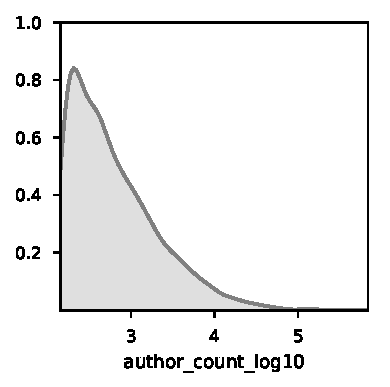
\includegraphics[width=\textwidth]{latex/kde/author_count_log10-active}
        \label{hist/sub:author}
    \end{subfigure}
    \hfill
    \begin{subfigure}[b]{0.49\textwidth}
        \centering
        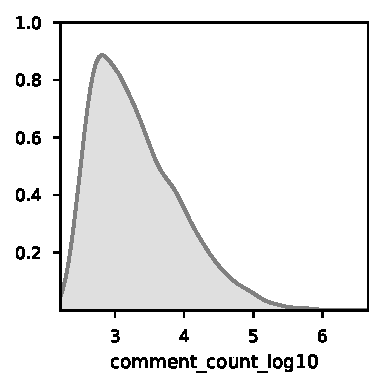
\includegraphics[width=\textwidth]{latex/kde/comment_count_log10-active.pdf}
        \label{hist/sub:comment}
    \end{subfigure}
    \hfill
    \begin{subfigure}[b]{0.49\textwidth}
        \centering
        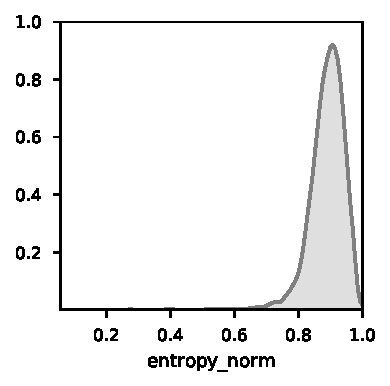
\includegraphics[width=\textwidth]{latex/kde/entropy_norm-active.pdf}
        \label{hist/sub:entropy}
    \end{subfigure}
    \hfill
    \begin{subfigure}[b]{0.49\textwidth}
        \centering
        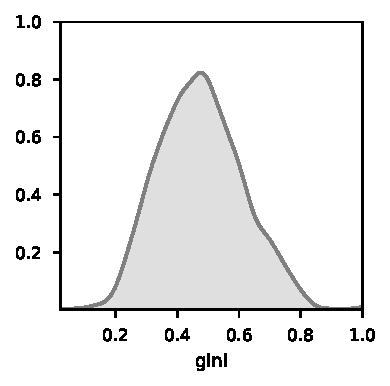
\includegraphics[width=\textwidth]{latex/kde/gini-active.pdf}
        \label{hist/sub:gini}
    \end{subfigure}
       \caption{Distributions of Subreddit-Level Statistics for Active Subreddit}
       \label{hists/sub:active}
\end{figure}
\begin{table}
\centering
\begin{tabular}{lrrrrrrr}
\toprule
{} &  entropy &  gini &  blau &  author\_count\_log10 &  comment\_count\_log10 &  entropy\_max &  entropy\_norm \\
\midrule
mean &    1.806 & 0.807 & 0.578 &               0.867 &                1.080 &        1.997 &         0.919 \\
std  &    1.817 & 0.212 & 0.380 &               0.881 &                1.047 &        2.029 &         0.102 \\
min  &    0.000 & 0.018 & 0.000 &               0.000 &                0.000 &        0.000 &         0.007 \\
25\%  &    0.000 & 0.655 & 0.000 &               0.000 &                0.301 &        0.000 &         0.892 \\
50\%  &    1.332 & 0.850 & 0.700 &               0.602 &                0.778 &        1.386 &         0.944 \\
75\%  &    2.797 & 1.000 & 0.920 &               1.342 &                1.653 &        3.091 &         0.986 \\
max  &   11.976 & 1.000 & 1.000 &               5.835 &                6.662 &       13.436 &         1.000 \\
\bottomrule
\end{tabular}
\caption{Descriptive Statistics for all Subreddits}
\label{table/all}
\end{table}
\begin{table}
\centering
\begin{tabular}{lrrrrrrr}
\toprule
{} &   mean &   std &   min &   25\% &    50\% &    75\% &    max \\
\midrule
author\_count\_log10  &  4.494 & 0.612 & 2.246 & 4.238 &  4.492 &  4.937 &  5.835 \\
blau                &  0.993 & 0.020 & 0.887 & 0.998 &  1.000 &  1.000 &  1.000 \\
comment\_count\_log10 &  4.878 & 0.671 & 2.650 & 4.526 &  4.858 &  5.306 &  6.662 \\
entropy             &  9.461 & 1.598 & 3.738 & 8.613 &  9.672 & 10.557 & 11.976 \\
entropy\_max         & 10.348 & 1.409 & 5.170 & 9.758 & 10.344 & 11.368 & 13.436 \\
entropy\_norm        &  0.910 & 0.064 & 0.712 & 0.901 &  0.934 &  0.946 &  0.983 \\
gini                &  0.511 & 0.101 & 0.278 & 0.459 &  0.517 &  0.577 &  0.801 \\
\bottomrule
\end{tabular}
\caption{Descriptive Statistics for Default Subreddits}
\label{table/defaults}
\end{table}
\begin{table}
\centering
\begin{tabular}{lrrrrrrr}
\toprule
{} &  mean &   std &   min &   25\% &   50\% &   75\% &    max \\
\midrule
entropy             & 5.724 & 1.138 & 0.318 & 4.913 & 5.493 & 6.325 & 11.976 \\
gini                & 0.476 & 0.137 & 0.021 & 0.378 & 0.471 & 0.567 &  1.000 \\
blau                & 0.986 & 0.034 & 0.070 & 0.986 & 0.992 & 0.996 &  1.000 \\
author\_count\_log10  & 2.798 & 0.524 & 2.158 & 2.377 & 2.667 & 3.089 &  5.835 \\
comment\_count\_log10 & 3.316 & 0.635 & 2.210 & 2.818 & 3.192 & 3.704 &  6.662 \\
entropy\_max         & 6.443 & 1.208 & 4.970 & 5.472 & 6.142 & 7.112 & 13.436 \\
entropy\_norm        & 0.889 & 0.062 & 0.056 & 0.862 & 0.897 & 0.927 &  1.000 \\
\bottomrule
\end{tabular}
\caption{Descriptive Statistics for Top Decile of Subreddits by Author Count}
\label{table/active}
\end{table}




\section{Author Concentration}

Similar to as we saw in Section \ref{subreddit vector}, for each author $a_i$ there are $n$ number of subreddits they commented in. For the $nth$ subreddit author $a_i$ there are $x_n$ number of comments, such that for each author we have the vector:

$$a_i = [x_1, x_2, \cdots x_n]$$

I then use this vector to calculate the three diversity measures as described in Sections \ref{entropy}, \ref{blau index}, and \ref{gini}. For each author we have the following measures:

\begin{itemize}
    \item number of subreddits
    \item number of comments
    \item author comment entropy
    \item author comment gini
    \item author comment blau
\end{itemize}


\subsection{General Trends}
Again focusing on active subreddits - what are the stats for these values of the author level?




\subsection{Author In-subreddit Ratio}
I also calculate the author in-subreddit ratio for each author, for each subreddit they commented in.
For author $A$ and subreddit $S$, if $x_S$ is the number of comments $A$ made in $S$ and $\sum A_i$ is the number of comments $A$ made across all subreddits, the author in-subreddit ratio is:

$$insub_A{}_S = \frac{x_s}{\sum A_i}$$

\subsection{Aggregating to Subreddit Level}
Section \ref{1.1} characterised subreddits by how authors behaved within subreddits. By now focusing on author activity across subreddits, we can look at how subreddits consists of authors who actor outside of their own space...

By aggregating author statistics to the subreddit level we can determine in certain subreddits tend to attract/consist of authors who are more or less diverse across the entire Reddit platform. For each subreddit I take the median value of each value across all authors who commented in that subreddit. For example, if 500 authors commented in r/ExampleSubreddit, I would take the median value of comment entropy for those 500 authors. I then repeat this for all variables, for all subreddits.

Table \ref{table/author-medians:all} shows the results for all subreddits. Again the count values are highly skewed across subreddits. The lower 75\% of subreddits have an average author subreddit count of 14.5 or less, and an average author comment count of 58 or less. However the maximum values are 7,996 and 1,245,236, respectively. 433 subreddits have these values because all were only commented in by 1 redditor, \textit{imguralbumbot}, a known bot account. Therefore, I again selected the top decile of subreddits by author count for further analysis.

Table \ref{table/author-medians:active} shows the results for the top decile of active subreddits. 

% Author-Level Figure

\begin{table}
\centering
\begin{tabular}{lrrrrrrrrrrrrrrrrrr}
\toprule
{} &  author\_count &  comment\_count &  entropy &   gini &   blau &  default\_x &  author\_count\_log10 &  comment\_count\_log10 &  entropy\_max &  entropy\_norm &  aut\_sub\_count &  aut\_com\_count &  aut\_com\_entropy &  aut\_com\_gini &  aut\_com\_blau &  aut\_insub &  aut\_sub\_count\_log10 &  aut\_com\_count\_log10 \\
\midrule
author\_count        &         1.000 &          0.900 &    0.418 & -0.073 &  0.054 &      0.488 &               0.428 &                0.375 &        0.428 &         0.023 &          0.056 &          0.039 &            0.056 &        -0.047 &         0.047 &     -0.024 &                0.059 &                0.054 \\
comment\_count       &         0.900 &          1.000 &    0.314 & -0.148 &  0.039 &      0.282 &               0.350 &                0.352 &        0.350 &        -0.041 &         -0.015 &         -0.004 &           -0.020 &        -0.016 &        -0.018 &      0.038 &               -0.011 &                0.009 \\
entropy             &         0.418 &          0.314 &    1.000 & -0.008 &  0.415 &      0.259 &               0.941 &                0.772 &        0.941 &         0.315 &          0.235 &          0.135 &            0.233 &        -0.129 &         0.192 &     -0.103 &                0.222 &                0.177 \\
gini                &        -0.073 &         -0.148 &   -0.008 &  1.000 &  0.206 &      0.020 &              -0.293 &               -0.608 &       -0.293 &         0.780 &          0.471 &          0.210 &            0.482 &        -0.037 &         0.389 &     -0.330 &                0.417 &                0.161 \\
blau                &         0.054 &          0.039 &    0.415 &  0.206 &  1.000 &      0.016 &               0.205 &                0.107 &        0.205 &         0.709 &          0.037 &          0.000 &            0.066 &        -0.053 &         0.074 &     -0.048 &                0.059 &                0.052 \\
default\_x           &         0.488 &          0.282 &    0.259 &  0.020 &  0.016 &      1.000 &               0.255 &                0.194 &        0.255 &         0.028 &          0.075 &          0.065 &            0.074 &        -0.064 &         0.061 &     -0.052 &                0.078 &                0.072 \\
author\_count\_log10  &         0.428 &          0.350 &    0.941 & -0.293 &  0.205 &      0.255 &               1.000 &                0.924 &        1.000 &        -0.018 &          0.129 &          0.094 &            0.115 &        -0.111 &         0.088 &     -0.013 &                0.121 &                0.135 \\
comment\_count\_log10 &         0.375 &          0.352 &    0.772 & -0.608 &  0.107 &      0.194 &               0.924 &                1.000 &        0.924 &        -0.294 &         -0.078 &          0.007 &           -0.113 &        -0.066 &        -0.113 &      0.162 &               -0.080 &                0.051 \\
entropy\_max         &         0.428 &          0.350 &    0.941 & -0.293 &  0.205 &      0.255 &               1.000 &                0.924 &        1.000 &        -0.018 &          0.129 &          0.094 &            0.115 &        -0.111 &         0.088 &     -0.013 &                0.121 &                0.135 \\
entropy\_norm        &         0.023 &         -0.041 &    0.315 &  0.780 &  0.709 &      0.028 &              -0.018 &               -0.294 &       -0.018 &         1.000 &          0.302 &          0.108 &            0.343 &        -0.059 &         0.305 &     -0.251 &                0.293 &                0.122 \\
aut\_sub\_count       &         0.056 &         -0.015 &    0.235 &  0.471 &  0.037 &      0.075 &               0.129 &               -0.078 &        0.129 &         0.302 &          1.000 &          0.873 &            0.916 &        -0.645 &         0.743 &     -0.611 &                0.922 &                0.836 \\
aut\_com\_count       &         0.039 &         -0.004 &    0.135 &  0.210 &  0.000 &      0.065 &               0.094 &                0.007 &        0.094 &         0.108 &          0.873 &          1.000 &            0.744 &        -0.755 &         0.588 &     -0.528 &                0.800 &                0.891 \\
aut\_com\_entropy     &         0.056 &         -0.020 &    0.233 &  0.482 &  0.066 &      0.074 &               0.115 &               -0.113 &        0.115 &         0.343 &          0.916 &          0.744 &            1.000 &        -0.729 &         0.935 &     -0.824 &                0.983 &                0.847 \\
aut\_com\_gini        &        -0.047 &         -0.016 &   -0.129 & -0.037 & -0.053 &     -0.064 &              -0.111 &               -0.066 &       -0.111 &        -0.059 &         -0.645 &         -0.755 &           -0.729 &         1.000 &        -0.762 &      0.815 &               -0.799 &               -0.915 \\
aut\_com\_blau        &         0.047 &         -0.018 &    0.192 &  0.389 &  0.074 &      0.061 &               0.088 &               -0.113 &        0.088 &         0.305 &          0.743 &          0.588 &            0.935 &        -0.762 &         1.000 &     -0.937 &                0.921 &                0.778 \\
aut\_insub           &        -0.024 &          0.038 &   -0.103 & -0.330 & -0.048 &     -0.052 &              -0.013 &                0.162 &       -0.013 &        -0.251 &         -0.611 &         -0.528 &           -0.824 &         0.815 &        -0.937 &      1.000 &               -0.837 &               -0.747 \\
aut\_sub\_count\_log10 &         0.059 &         -0.011 &    0.222 &  0.417 &  0.059 &      0.078 &               0.121 &               -0.080 &        0.121 &         0.293 &          0.922 &          0.800 &            0.983 &        -0.799 &         0.921 &     -0.837 &                1.000 &                0.902 \\
aut\_com\_count\_log10 &         0.054 &          0.009 &    0.177 &  0.161 &  0.052 &      0.072 &               0.135 &                0.051 &        0.135 &         0.122 &          0.836 &          0.891 &            0.847 &        -0.915 &         0.778 &     -0.747 &                0.902 &                1.000 \\
\bottomrule
\end{tabular}
\caption{Correlations for Active subreddits}
\label{table/corr:active}
\end{table}
\begin{table}
\centering
\begin{tabular}{lrrrrrr}
\toprule
{} &  aut\_sub\_count &  aut\_com\_count &  aut\_com\_entropy &  aut\_com\_gini &  aut\_com\_blau &     aut\_insub \\
\midrule
mean &     213.520226 &   5.411813e+03 &         1.645732 &     -1.954438 &      0.597107 &  2.619530e-01 \\
std  &     915.413325 &   7.113781e+04 &         1.452357 &      0.476181 &      0.301553 &  3.383600e-01 \\
min  &       1.000000 &   1.000000e+00 &         0.000000 &     -3.000000 &      0.000000 &  8.030606e-07 \\
25\%  &       3.000000 &   6.000000e+00 &         0.693147 &     -2.018923 &      0.463138 &  2.941176e-02 \\
50\%  &       6.500000 &   1.950000e+01 &         1.428056 &     -1.788352 &      0.687500 &  9.638554e-02 \\
75\%  &      14.500000 &   5.800000e+01 &         2.086235 &     -1.650794 &      0.820000 &  3.333333e-01 \\
max  &    7996.000000 &   1.245236e+06 &         7.672562 &     -1.089127 &      0.998361 &  1.000000e+00 \\
\bottomrule
\end{tabular}
\caption{Distribution of Author Medians for All Subreddits}
\label{table/author-medians:all}
\end{table}
\begin{table}
\centering
\begin{tabular}{lrrrrrr}
\toprule
{} &  aut\_sub\_count &  aut\_com\_count &  aut\_com\_entropy &  aut\_com\_gini &  aut\_com\_blau &  aut\_insub \\
\midrule
mean &          8.180 &         25.049 &            1.530 &        -1.785 &         0.693 &      0.163 \\
std  &          5.122 &         17.728 &            0.527 &         0.211 &         0.154 &      0.177 \\
min  &          1.000 &          1.000 &            0.000 &        -3.000 &         0.000 &      0.009 \\
25\%  &          5.000 &         13.000 &            1.223 &        -1.833 &         0.640 &      0.059 \\
50\%  &          7.000 &         20.000 &            1.514 &        -1.746 &         0.720 &      0.111 \\
75\%  &         10.000 &         31.500 &            1.871 &        -1.667 &         0.793 &      0.188 \\
max  &         33.000 &        161.500 &            2.867 &        -1.507 &         0.913 &      1.000 \\
\bottomrule
\end{tabular}
\caption{Distribution of Author Medians for Active Subreddits}
\label{table/author-medians:active}
\end{table}
\begin{figure}
    \centering
    \begin{subfigure}[b]{0.49\textwidth}
        \centering
        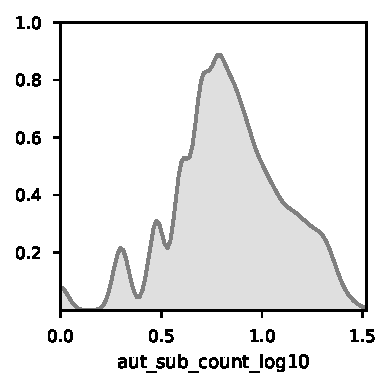
\includegraphics[width=\textwidth]{latex/kde/aut_sub_count_log10-active}
        \label{hist/aut:sub}
    \end{subfigure}
    \hfill
    \begin{subfigure}[b]{0.49\textwidth}
        \centering
        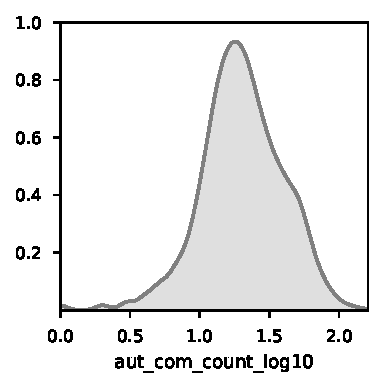
\includegraphics[width=\textwidth]{latex/kde/aut_com_count_log10-active.pdf}
        \label{hist/aut:com}
    \end{subfigure}
    \hfill
    \begin{subfigure}[b]{0.49\textwidth}
        \centering
        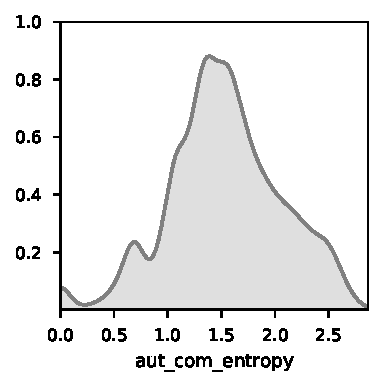
\includegraphics[width=\textwidth]{latex/kde/aut_com_entropy-active.pdf}
        \label{hist/aut:entropy}
    \end{subfigure}
    \hfill
    \begin{subfigure}[b]{0.49\textwidth}
        \centering
        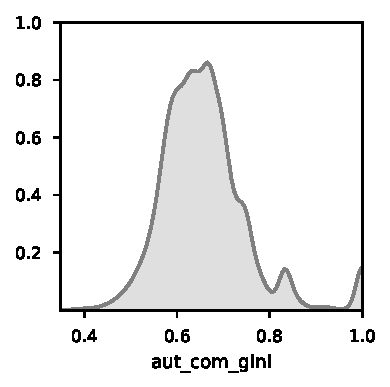
\includegraphics[width=\textwidth]{latex/kde/aut_com_gini-active.pdf}
        \label{hist/aut:gini}
    \end{subfigure}
    \hfill
    \begin{subfigure}[b]{0.49\textwidth}
        \centering
        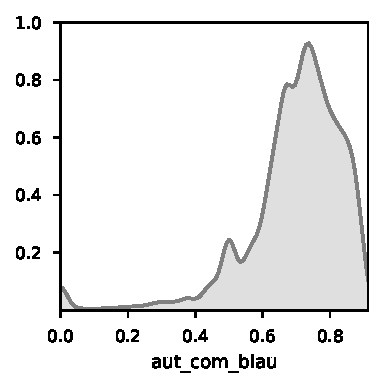
\includegraphics[width=\textwidth]{latex/kde/aut_com_blau-active.pdf}
        \label{hist/aut:blau}
    \end{subfigure}
    \hfill
    \begin{subfigure}[b]{0.49\textwidth}
        \centering
        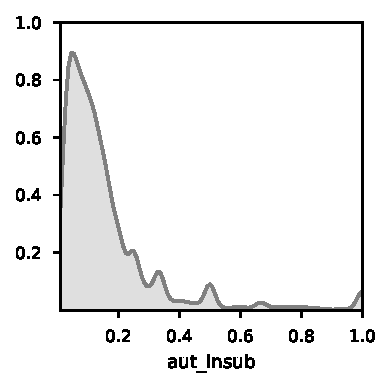
\includegraphics[width=\textwidth]{latex/kde/aut_insub-active.pdf}
        \label{hist/aut:insub}
    \end{subfigure}
    \caption{Distributions of Author-Level Statistics for Active Subreddits}
    \label{hists/aut:active}
\end{figure}



\section{Political Case Studies}


Currently I have 8 case study politically-oriented subreddits. There are loosely ordered from most politically right wing to most left wing, with quoted community description:

\begin{enumerate}
    \item \href{https://www.reddit.com/r/The_Donald}{r/The\_Donald: ``The\_Donald is a never-ending rally dedicated to the 45th President of the United States, Donald J. Trump."}
    
    \item \href{https://www.reddit.com/r/Conservative}{r/Libertarian: ``A place to discuss free market libertarianism and related topics, and share things that would be of interest to libertarians.''}
    
    \item \href{https://www.reddit.com/r/Conservative}{r/Conservative: ``The place for Conservatives on Reddit." }
    
    \item \href{https://www.reddit.com/r/politics}{r/politics: ``/r/Politics is for news and discussion about U.S. politics."}
    
    \item \href{https://www.reddit.com/r/Conservative}{r/changemyview: ``A place to post an opinion you accept may be flawed, in an effort to understand other perspectives on the issue. Enter with a mindset for conversation, not debate."}
    
    \item \href{https://www.reddit.com/r/socialism}{r/socialism: ``This is a community to discuss current events in our world from an anti-capitalist perspective and to provide clarity to socialist ideas"}
    \item \href{https://www.reddit.com/r/SandersForPresident}{r/SandersForPresident: ``Run Bernie Run!"}
    \item \href{https://www.reddit.com/r/Conservative}{r/LateStageCaptialism: ``A One-Stop-Shop for Evidence of our Social, Moral and Ideological Rot.''}
\end{enumerate}

Both r/The\_Donald and r/LateStageCapitalism clearly state that they will remove content and ban users who dissent from their respective general opinions, i.e. Pro-Trump or anti-capitalist sentiment. As such they can be considered to tacitly encourage echo chamber behaviours. At this point I take them to be my examples of a right wing and a left wing echo chamber. r/politics is the only default subreddit on the list. It is a place for general discussions on US politics, with no set political stance, thus I've place it in the middle of the list. r/changemyview was created to be an "anti-echo chamber", to actively encourage people with opposing opinions to debate each other. I therefore place it in the middle of the list. The r/Libertarian, r/Conservative, and r/socialism are all generalist subreddits which each favour their named viewpoints. r/SandersforPresident was originally inteded to supporter Bernie Sander's run for the US Presidency in 2016. It is fairly active, and likely to see a resurgence heading into 2020.


% Political Visuals
\begin{figure}
    \centering
    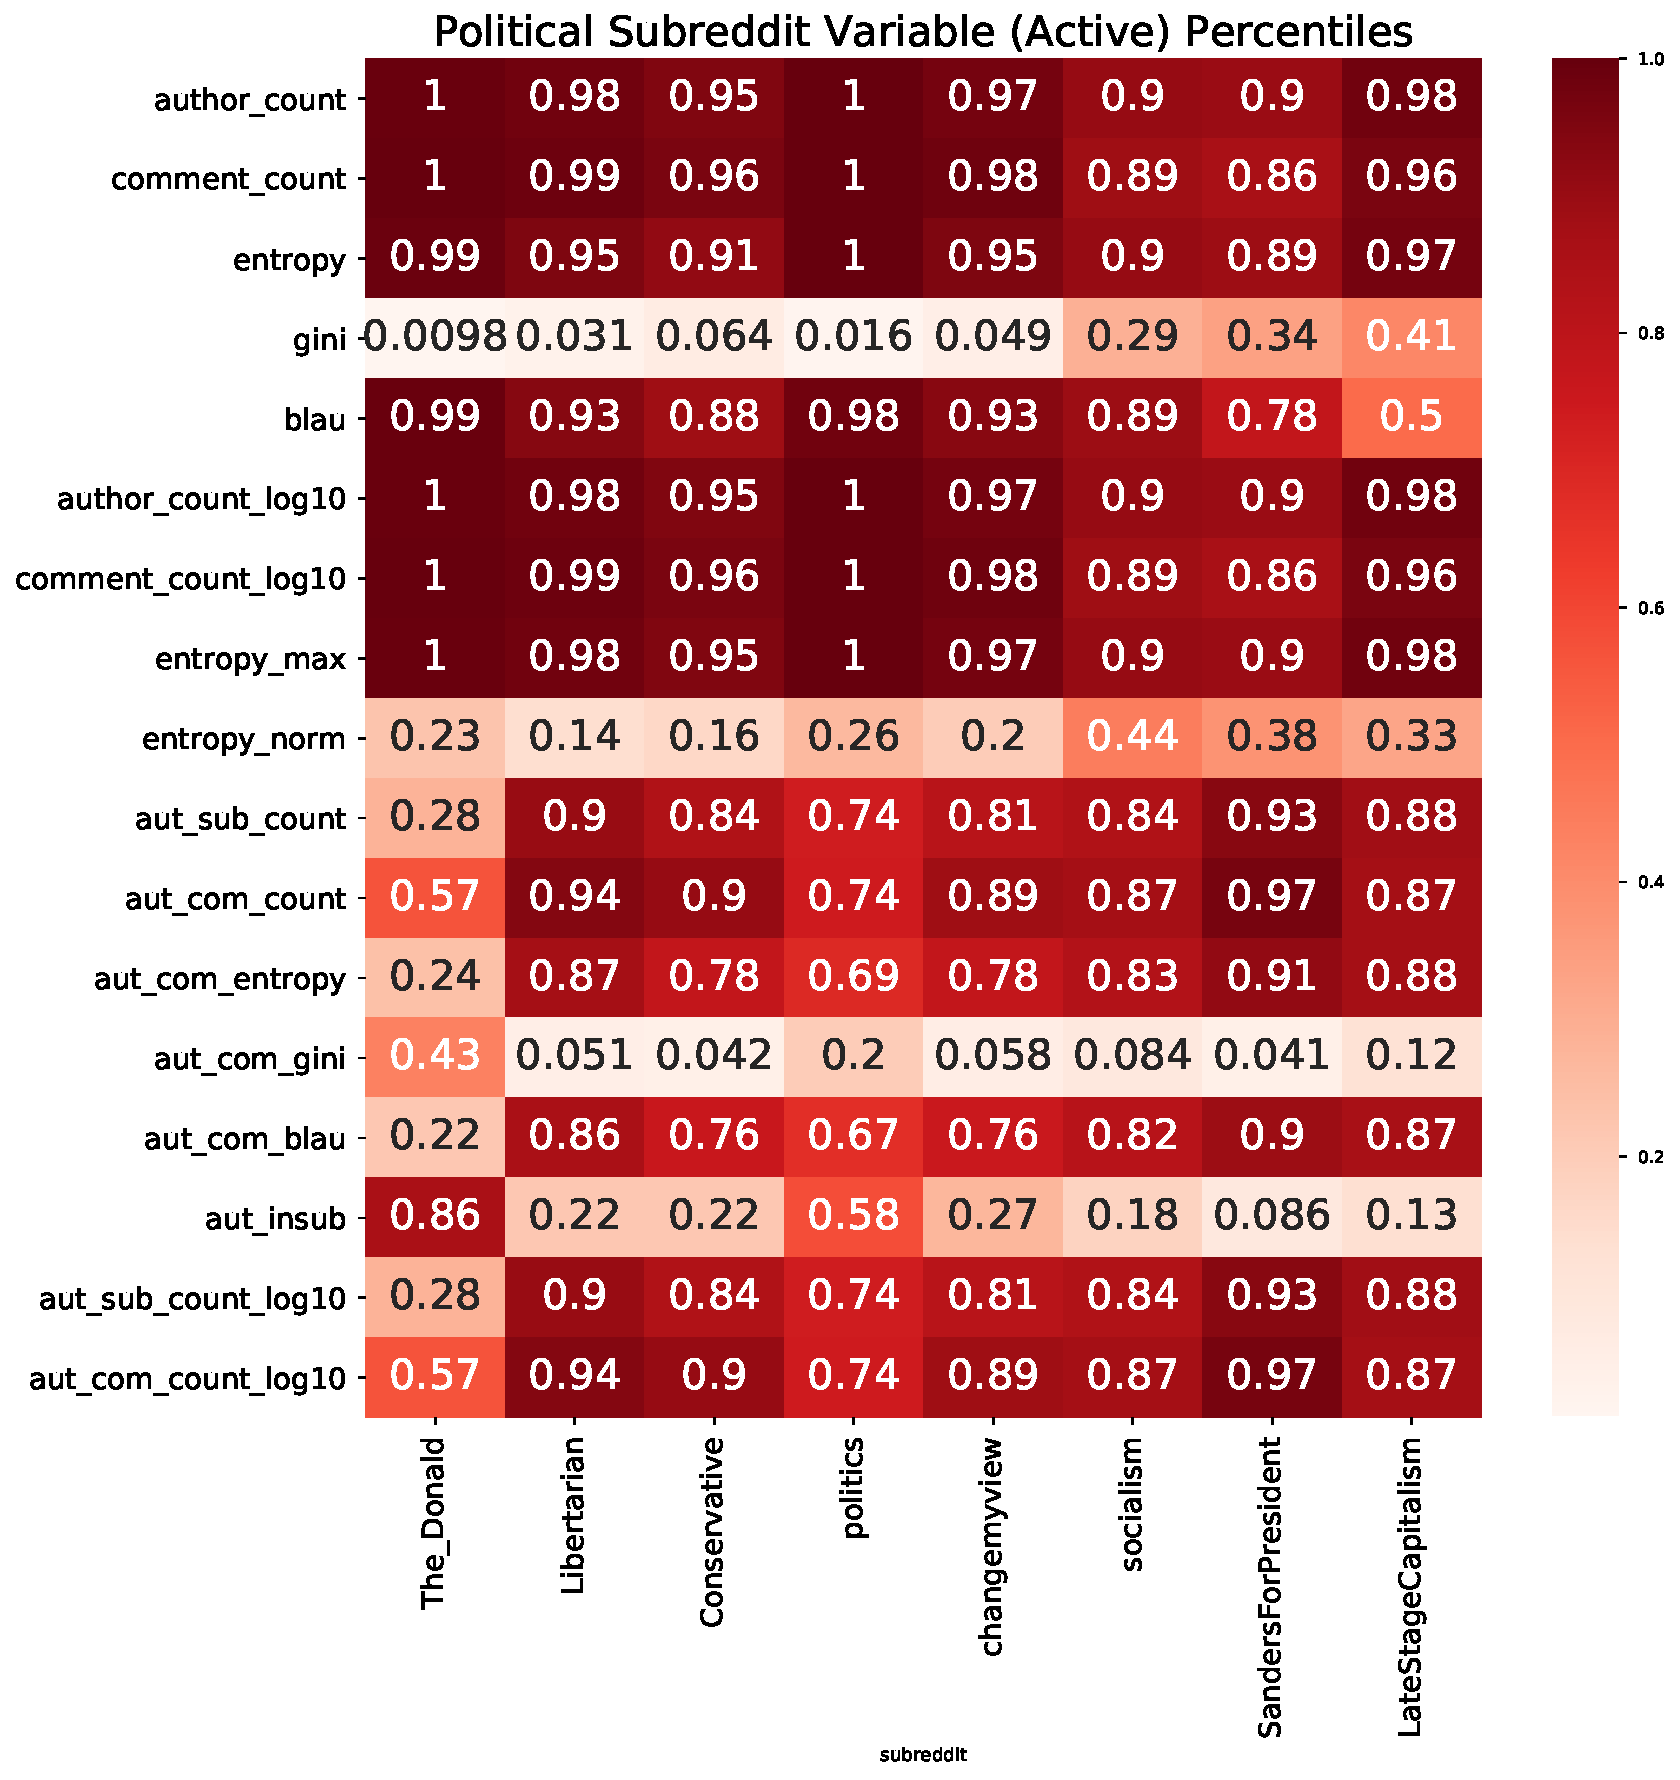
\includegraphics[width=\textwidth]{latex/pol-heatmap.pdf}
    \caption{Political Subreddit Variable Percentiles}
    \label{pol-heatmap}
\end{figure}

The subreddits list so far we selected from a manual search of the 500 (or 1000?) most active subreddits during a previous sampling stage. This list can be easily extended as more approiate politically-oriented subreddits come to my attention.

Figure \ref{pol-heatmap} shows the percentiles for  these political subreddits, compared to the 8094 active subreddits. The raw data can bee seen in Table \ref{pol-heatmap}. All of the subreddits are the in 90th or higher percentile by author count, and 96th percentile for comment count (with the exception of r/socialism (89th) and r/SandersForPresident (86th). 

\subsection{Interpretation}






\begin{landscape}
\begin{table}
\centering
\begin{tabular}{lrrrrrrrr}
\toprule
subreddit &  The\_Donald &  Libertarian &  Conservative &   politics &  changemyview &  socialism &  SandersForPresident &  LateStageCapitalism \\
\midrule
author\_count        &    44917.00 &     13249.00 &       6468.00 &  136116.00 &      11215.00 &    3664.00 &              3445.00 &             15091.00 \\
comment\_count       &   784104.00 &    107933.00 &      42927.00 & 1624275.00 &      86088.00 &   13777.00 &             11509.00 &             43005.00 \\
entropy             &        9.20 &         7.95 &          7.41 &      10.21 &          7.95 &       7.30 &                 7.18 &                 8.41 \\
gini                &        0.20 &         0.25 &          0.28 &       0.22 &          0.26 &       0.39 &                 0.41 &                 0.44 \\
blau                &        1.00 &         1.00 &          1.00 &       1.00 &          1.00 &       1.00 &                 1.00 &                 0.99 \\
author\_count\_log10  &        4.65 &         4.12 &          3.81 &       5.13 &          4.05 &       3.56 &                 3.54 &                 4.18 \\
comment\_count\_log10 &        5.89 &         5.03 &          4.63 &       6.21 &          4.93 &       4.14 &                 4.06 &                 4.63 \\
entropy\_max         &       10.71 &         9.49 &          8.77 &      11.82 &          9.33 &       8.21 &                 8.14 &                 9.62 \\
entropy\_norm        &        0.86 &         0.84 &          0.84 &       0.86 &          0.85 &       0.89 &                 0.88 &                 0.87 \\
aut\_sub\_count       &        5.00 &        16.00 &         13.00 &      10.00 &         12.00 &      13.00 &                18.00 &                15.00 \\
aut\_com\_count       &       22.00 &        57.00 &         50.00 &      31.00 &         47.00 &      45.00 &                66.00 &                45.00 \\
aut\_com\_entropy     &        1.21 &         2.18 &          1.94 &       1.75 &          1.93 &       2.06 &                 2.30 &                 2.18 \\
aut\_com\_gini        &        0.64 &         0.53 &          0.53 &       0.59 &          0.54 &       0.55 &                 0.53 &                 0.57 \\
aut\_com\_blau        &        0.62 &         0.83 &          0.80 &       0.77 &          0.80 &       0.82 &                 0.85 &                 0.84 \\
aut\_insub           &        0.27 &         0.05 &          0.05 &       0.13 &          0.06 &       0.05 &                 0.03 &                 0.04 \\
aut\_sub\_count\_log10 &        0.70 &         1.20 &          1.11 &       1.00 &          1.08 &       1.11 &                 1.26 &                 1.18 \\
aut\_com\_count\_log10 &        1.34 &         1.76 &          1.70 &       1.49 &          1.67 &       1.65 &                 1.82 &                 1.65 \\
\bottomrule
\end{tabular}
\caption{Political Subreddit Results}
\label{table/pol}
\end{table}
\end{landscape}





\section{Proposed Robustness Checks}

\subsection{Change Subset Threshold}

Compare results to those for the top 5\% or top 20\& of authors?

\subsection{Longitudinal Variation}

Show stability of variables over time

\subsection{Subsetting by Comment Count}

Re-run analysis on another month


\end{document}
